En esta sección del informe realizaremos experimentos con todos los algoritmos implementados evaluando tanto la complejidad como la eficacia de las heurísticas implementadas.

Para lo primero graficamos los ciclos insumidos en función de la cantidad de nodos para varios grafos generados aleatoriamente. Los resultados fueron los siguientes:

\begin{figure}[H]
\centering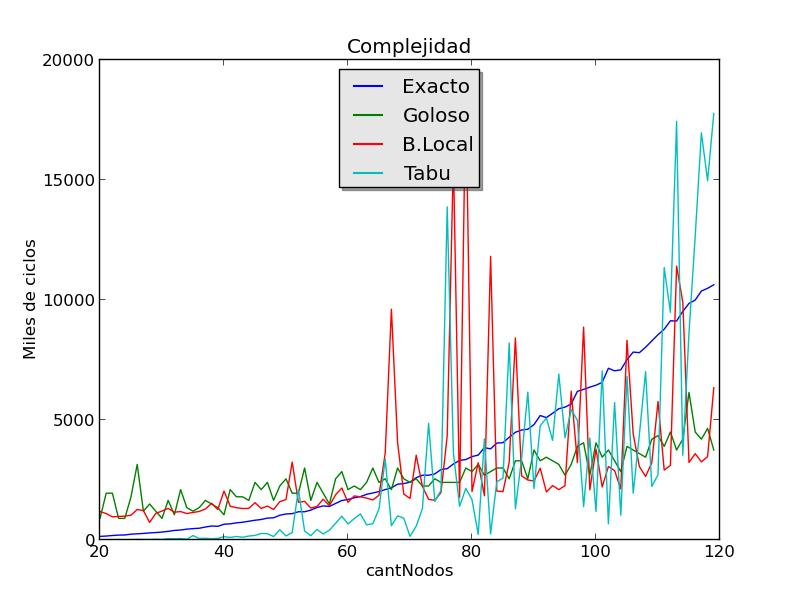
\includegraphics[width=11 cm]{experimentacion/complejidad.jpg}
\caption{Cantidad de ciclos insumidos en función de la cantidad de nodos en el grafo.}
\end{figure}

Para lo segundo decidimos utilizar un conjunto de pruebas conformado por tests de la cátedra sumándole varias instancias de casos random con grafos que van de 1 a 120 nodos. Los resultados obtenidos para cada test fueron comparados con los devueltos por el algoritmo exacto de la siguiente manera: \\

$\forall i \in pruebas \sum{\frac{res\_heurística[i]}{res\_exacto[i]}} * 100 \ = \ efectividad\_heuristica$ (medida en \%)
$res\_exacto$ y $res\_heurística$ es el cardinal de la frontera devuelta por el algoritmo exacto y la heurística respectivamente.

Considerando que la efectividad del algoritmo exacto es 100$\%$, la efectividad de cada heurística puede apreciarse en el siguiente gráfico:

\begin{figure}[H]
\centering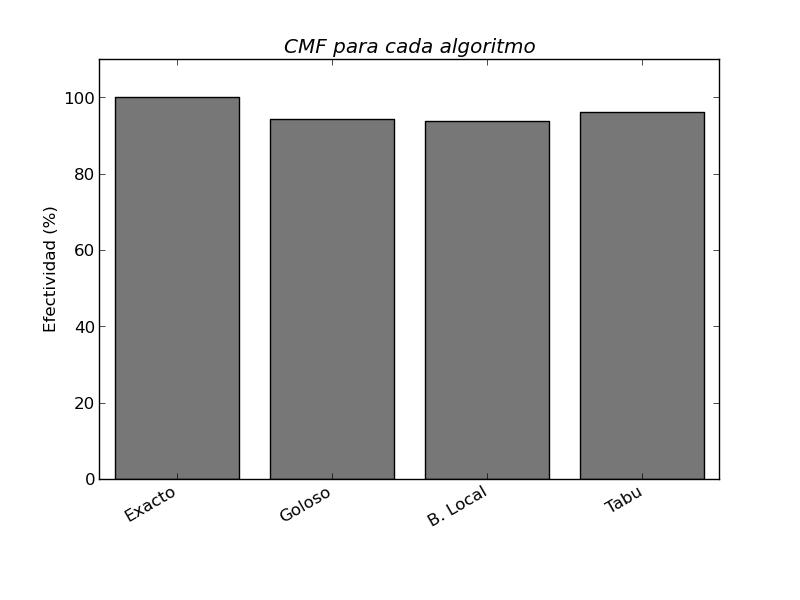
\includegraphics[width=11 cm]{experimentacion/efectividad.jpg}
\caption{Cantidad de ciclos insumidos en función de la cantidad de nodos en el grafo.}
\end{figure}

Como puede observarse, la efectividad de las heurísticas se encuentran por arriba del 90\%. La heurística que mejor funcionó fue la Tabú, seguido por la Búsqueda Local y la golosa. Era de esperar que el Tabú search fuera mejor que la búsqueda local ya que el primer algoritmo es una modificación del segundo con la ventaja de que puede salir de los óptimos locales. 






